\documentclass{article}
\usepackage[margin=1in,a4paper]{geometry}
\usepackage[utf8]{inputenc}
\usepackage[cyr]{aeguill}
\usepackage[francais]{babel}
\usepackage{hyperref}
\usepackage{amsmath}
\usepackage{gensymb}
\usepackage{enumitem,amssymb}
\newlist{checks}{itemize}{2}
\setlist[checks]{label=$\square$}
\usepackage{graphicx}
\usepackage{amsthm}
\usepackage{amsfonts}
\usepackage{multicol}
\usepackage{pgfplots}
\pgfplotsset{compat=newest}
\usetikzlibrary{calc}
\usepackage{mathtools}
\usepackage{array}
\usepackage[T1]{fontenc}
\usepackage{lmodern}
\usepackage{tabularx}
\usepackage{fancyhdr}
\usepackage{pst-func}
\usepackage{xcolor}
\usepackage{nicefrac}
\usepackage{mdframed}
\usepackage[boxed,vlined]{algorithm2e}
\usepackage{cleveref}
\newcommand{\Lim}[1]{\raisebox{0.5ex}{\scalebox{1}{$\displaystyle \lim_{#1}\;$}}}
\usepackage{float}
%\usepackage[top=2.5cm, bottom=2cm, left=2cm, right=2cm, showframe]{geometry}
\usepackage[top=2.5cm, bottom=2cm, left=2cm, right=2cm]{geometry}
\newcommand{\N}{\mathbb{N}}
\newcommand{\R}{\mathbb{R}}
\renewcommand{\C}{\mathbb{C}}
\renewcommand{\P}{\mathbb{P}}
\newcommand{\w}{\omega}
\newcommand{\p}{\partial}
\newcommand{\cross}{\times}
\newcommand{\Col}{\text{Col}}
\newcommand{\Tr}{\text{Tr}}
\newcommand{\bigzero}{\makebox(0,0){\text{\huge0}}}
\DeclareMathOperator{\Ima}{Im}
\DeclareMathOperator{\Vect}{Vect}
\usepackage{mathtools, stmaryrd}
\usepackage{xparse} \DeclarePairedDelimiterX{\Iintv}[1]{\llbracket}{\rrbracket}{\iintvargs{#1}}
\NewDocumentCommand{\iintvargs}{>{\SplitArgument{1}{,}}m}
{\iintvargsaux#1} %
\NewDocumentCommand{\iintvargsaux}{mm} {#1\mkern1.5mu..\mkern1.5mu#2}
\newcommand{\Cc}{{\mathbb{C}}}
\newcommand{\Ct}{\Cc^\times}
\newcommand{\Hh}{{\mathbb{H}}}
\newcommand{\Nn}{{\mathbb{N}}}
\newcommand{\Zz}{{\mathbb{Z}}}
\newcommand{\Zzn}{\Zz/n\Zz}
\newcommand{\ZzNt}{(\Zz/N\Zz)^\times}%quotient 
\newcommand{\Rr}{{\mathbb{R}}}
\newcommand{\Rt}{{\Rr^\times}}
\newcommand{\Qt}{{\Qq^\times}}
\newcommand{\Qq}{{\mathbb{Q}}}
% Custom titling
\usepackage{titling}
\usepackage{tcolorbox}

\title{\textbf{Analyse Avancée -- Corrigé 2}}

\renewcommand{\maketitlehookb}{
\begin{center}

\includegraphics[width=2cm]{Cours/assets/imgs/logo-round.png}
\end{center}
}

\author{Students 4 Students}
\date{Septembre 2023}

% Exercises environment and styling
\usepackage{amsthm}
\newtheoremstyle{exercice}%
    {3pt}% Space above
    {3pt}% Space below
    {\large}% Body font
    {}% Indent amount
    {\bfseries}% Theorem head font
    {}% Punctuation after theorem heading
    {\newline}% Space after theorem heading
    {\thmname{#1}\thmnumber{ #2}\thmnote{: #3}}% Theorem head spec (can be left empty, meaning ‘normal’)
\theoremstyle{exercice}
\newtheorem{exercice}{Exercice}


\begin{document}

% Header
\pagestyle{fancy}
\fancyhead[L]{Students 4 Students}
\fancyhead[C]{\textit{Analyse avancée - Corrigé 2}}
\fancyhead[R]{Septembre 2023}

\maketitle



\begin{exercice}[Limites usuelles]
    Les limites donnent les résultats suivants:
\begin{enumerate}
    \item Pour $x_n=n$: \\
    On observe trivialement qu'elle tend vers l'infini. Pour le démontrer facilement, il suffit de montrer qu'elle est croissante et non bornée. La croissance est évidente. Pour montrer qu'elle est bornée, si l'on suppose parl'absurde qu'elle est bornée par un nombre $k\in \Rr$, alors on observe que $x_{k+1}>k$. Ainsi elle n'est pas bornée et est croissante: elle diverge vers l'infini.
    \item Pour $x_n=n^p$, $p>0$: \\
    Démontrons qu'elle tend vers l'infini. Premièrement elle est croissante. De plus, si l'on suppose qu'elle est bornée par un nombre $k\in \Rr$, alors on observe que $x_{t}>k$, $t=(k+1)^\tfrac{1}{p}$. Ainsi elle n'est pas bornée et est croissante: elle diverge vers l'infini.
    \item Pour $x_n=n^p$, $p\leq0$: \\
    Si $p=0$, on a $x_n=1$ donc la limite est 1.
    Pour $p<0$, démontrons qu'elle tend vers 0. Il est possible de le faire en montrant qu'elle est bornée par 0 et décroissante. Autrement, en appliquant le définition, trouvons le rang $N$ pour un $\varepsilon>0$ fixé tel que $|x_N|<\varepsilon$.

    \begin{equation}
    |x_N|<\varepsilon \iff N^p<\varepsilon \iff \frac{1}{\varepsilon}<N^{|p|}\iff \left( \frac{1}{\varepsilon}\right)^{\tfrac{1}{|p|}} <N
    \end{equation}
    
    Nous avons trouvé un rang à partir duquel la propriété est vraie. La suite tend bien vers 0.
    \item Pour $x_n=a n^p$:\\
    Si $a=0$, la suite vaudra 0 donc admet 0 comme limite. Sinon, si $p=0$ la suite vaut $a$ et l'admet donc comme limite. Sinon, si $p$ est négatif, la suite tend vers 0 comme vu à travers de l'exercice précédent. Si $p$ est positif, la suite tend vers $\text{sgn}(a) \infty$.
    \item Pour $x_n=\frac{n^p}{n^q}$:\\
    On a $x_n=n^{p-q}$ et retournons à la question précédente et observons que cela dépend du signe de $p-q$.
    \item Pour $x_n=\dfrac{a_pn^p+a_{p-1}n^{p-1}+...+a_0}{b_qn^q+b_{q-1}n^{q-1}+...+b_0}$:\\
    Nous allons utiliser les précédentes règles démontrées.\\ Premièrement, $x_n=\dfrac{a_pn^p}{b_qn^q}\cdot\dfrac{1+\sum_{k=1}^{p-1} \frac{a_k}{a_p}n^{k-p}}{1+\sum_{k=1}^{q-1} \frac{b_k}{b_q}n^{k-q}}$. La fraction de droite tend vers 1 car chaque somme tend vers 0 de par le fait que $k-p$ et $k-q$ sont toujours négatifs. Ainsi, on a $\underset{{n\to\infty}}{lim} x_n=\underset{{n\to\infty}}{lim} \dfrac{a_pn^p}{b_qn^q}=\dfrac{a_p}{b_q}~~\underset{{n\to\infty}}{lim} \dfrac{n^p}{n^q}$ que l'on a démontré dans la question précédente.  
\end{enumerate}


\end{exercice}


\begin{exercice}[Sous-suites, Principe des deux gendarmes]
    
\textbf{Sous-suites}

\textbf{a)} \\

\begin{figure}[H]
    \centering
    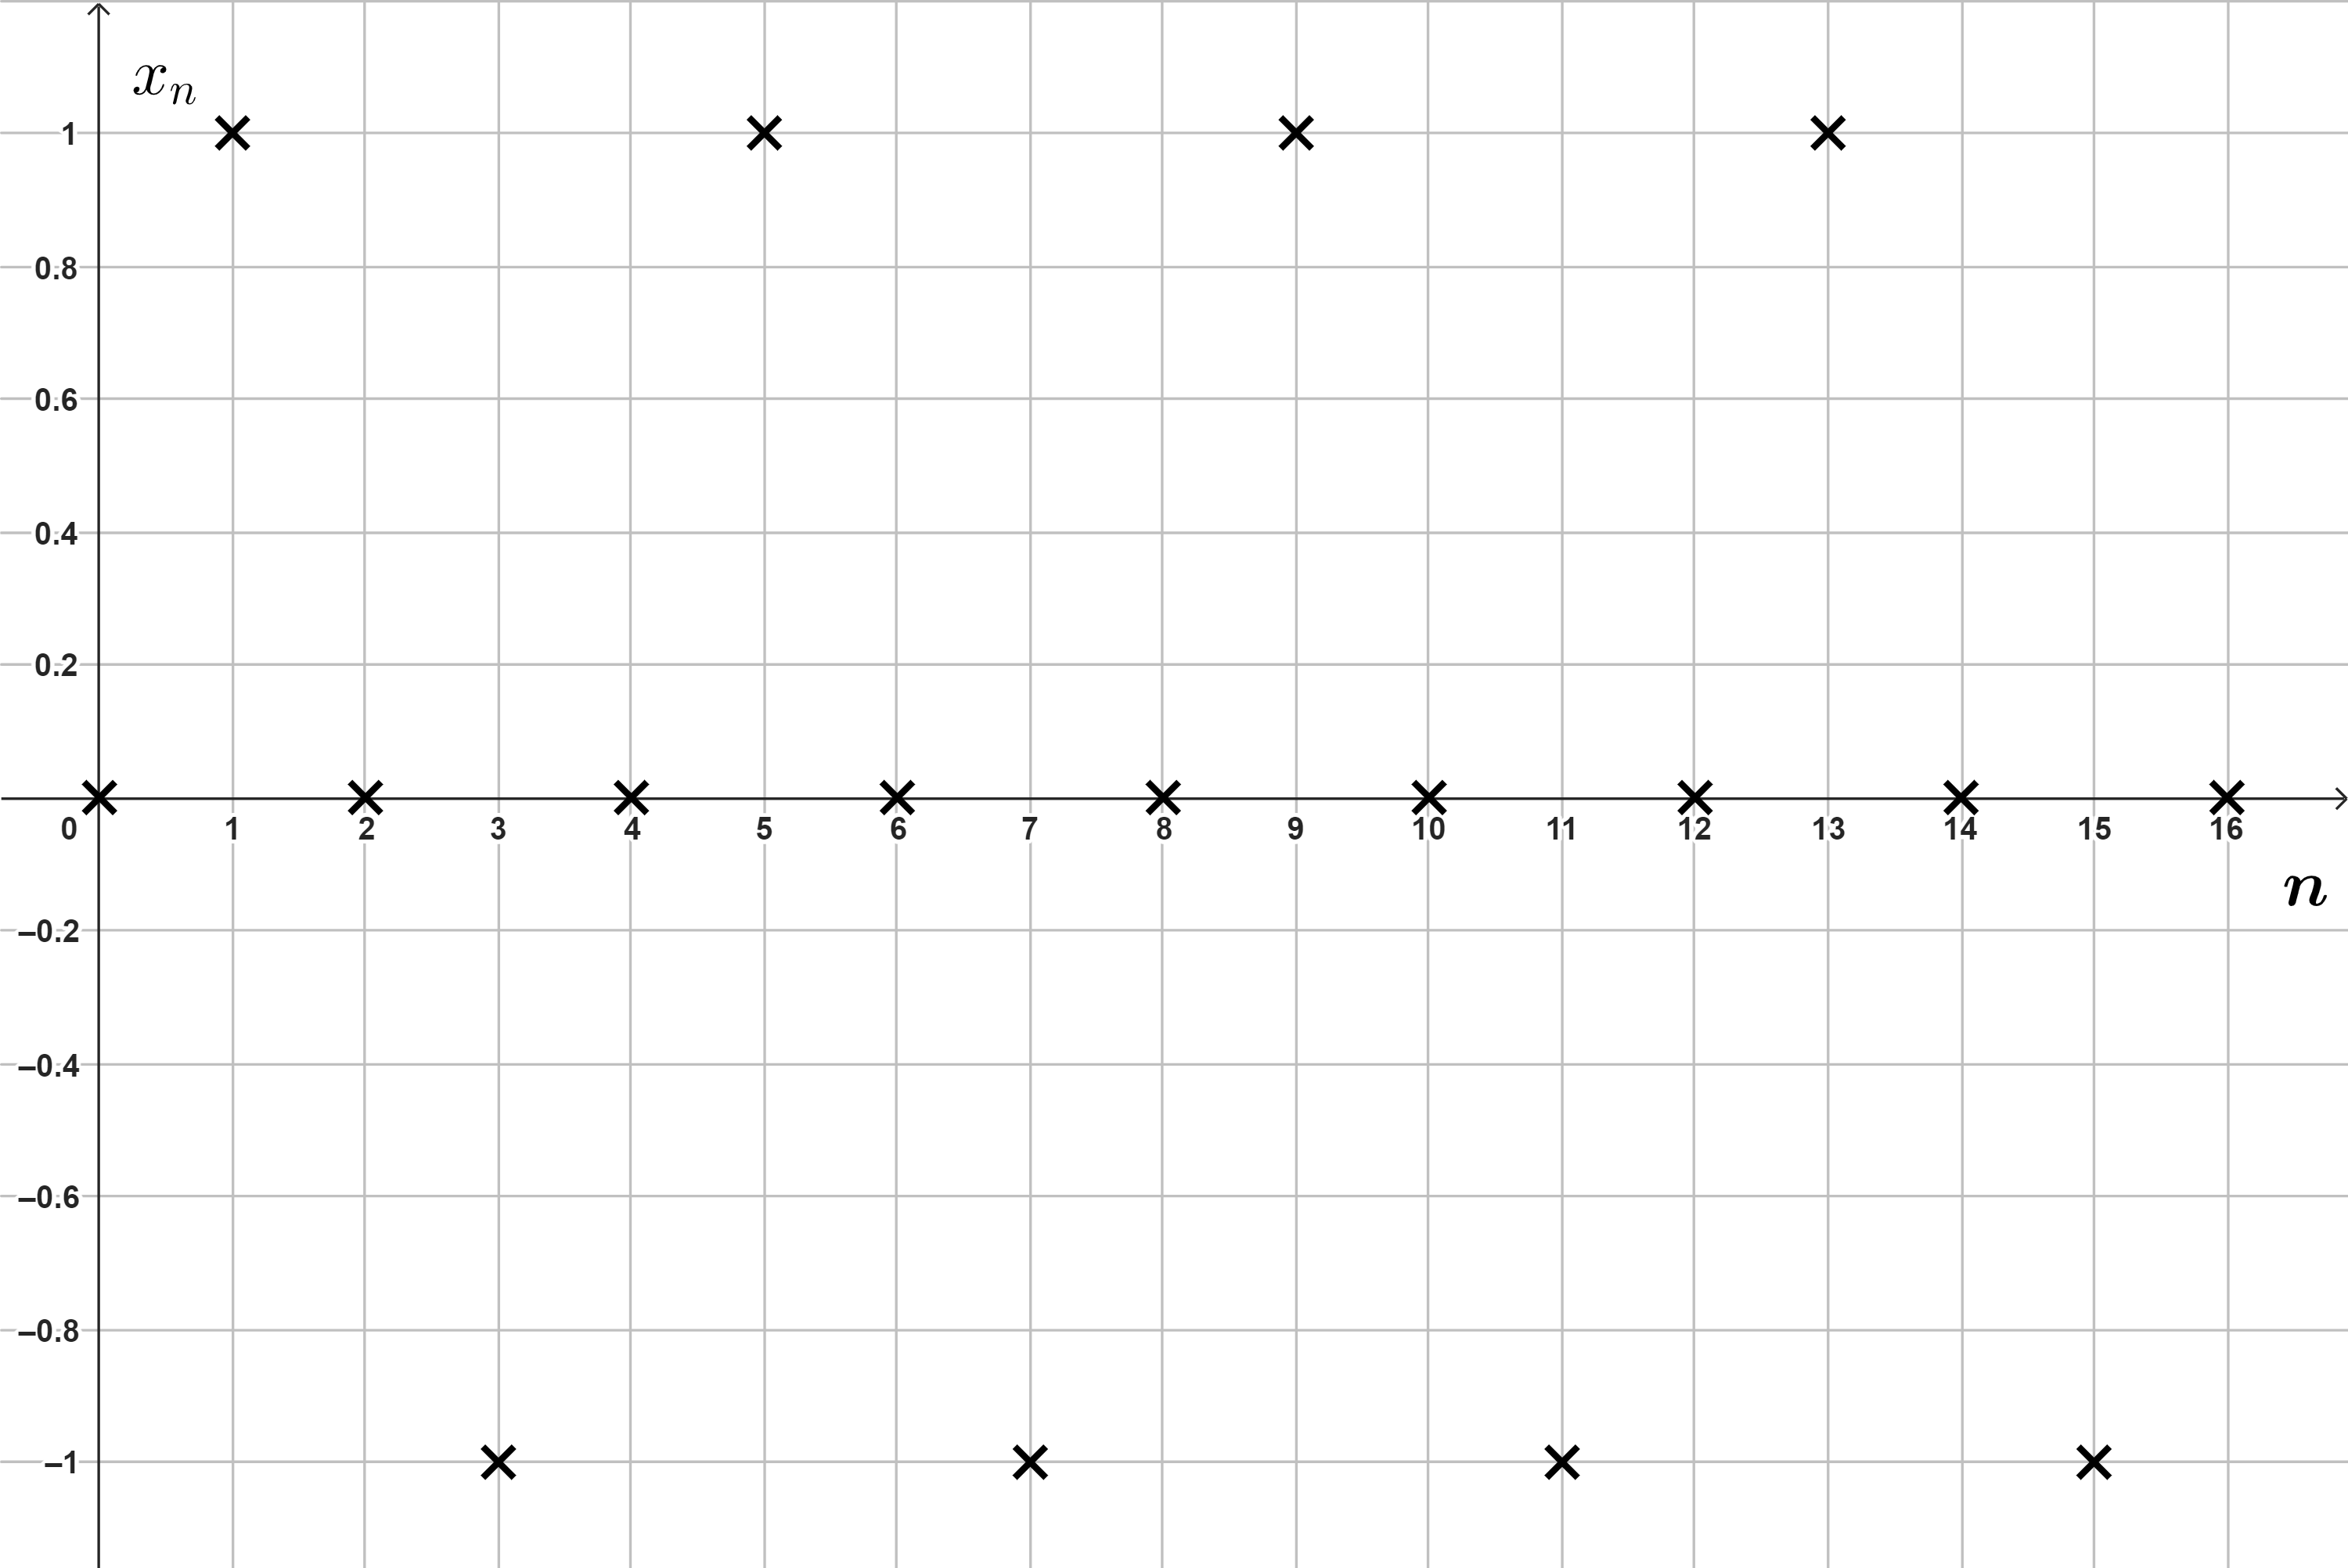
\includegraphics[scale=0.7]{Exercices/schema2.png}
    \caption{Representation des premiers termes de la suite $x_n=sin(n\frac{\pi}{2}$.}
    \label{fig:enter-label}
\end{figure}

\textbf{b)} La suite $x_n$ ne converge pas, mais la sous-suite $x_{2n}$ converge vers 0 (elle est d'ailleurs même constante: elle vaut toujours 0).\\

\textbf{c)} Pour rappel, les limites inférieure et supérieure d'une suite sont respectivement l'infimum et le suprémum des limites des sous-suites de $x_n$. Notre dessin au point \textbf{a)} nous montre que la limite inférieure est de -1 (obtenue par exemple avec la sous-suite $x_{1+4n}$) et la limite supérieure de 1 (obtenue par exemple avec la sous-suite $x_{3+4n}$). \\

\textbf{d)} La suite converge vers 0. \\


\begin{figure}[H]
    \centering
    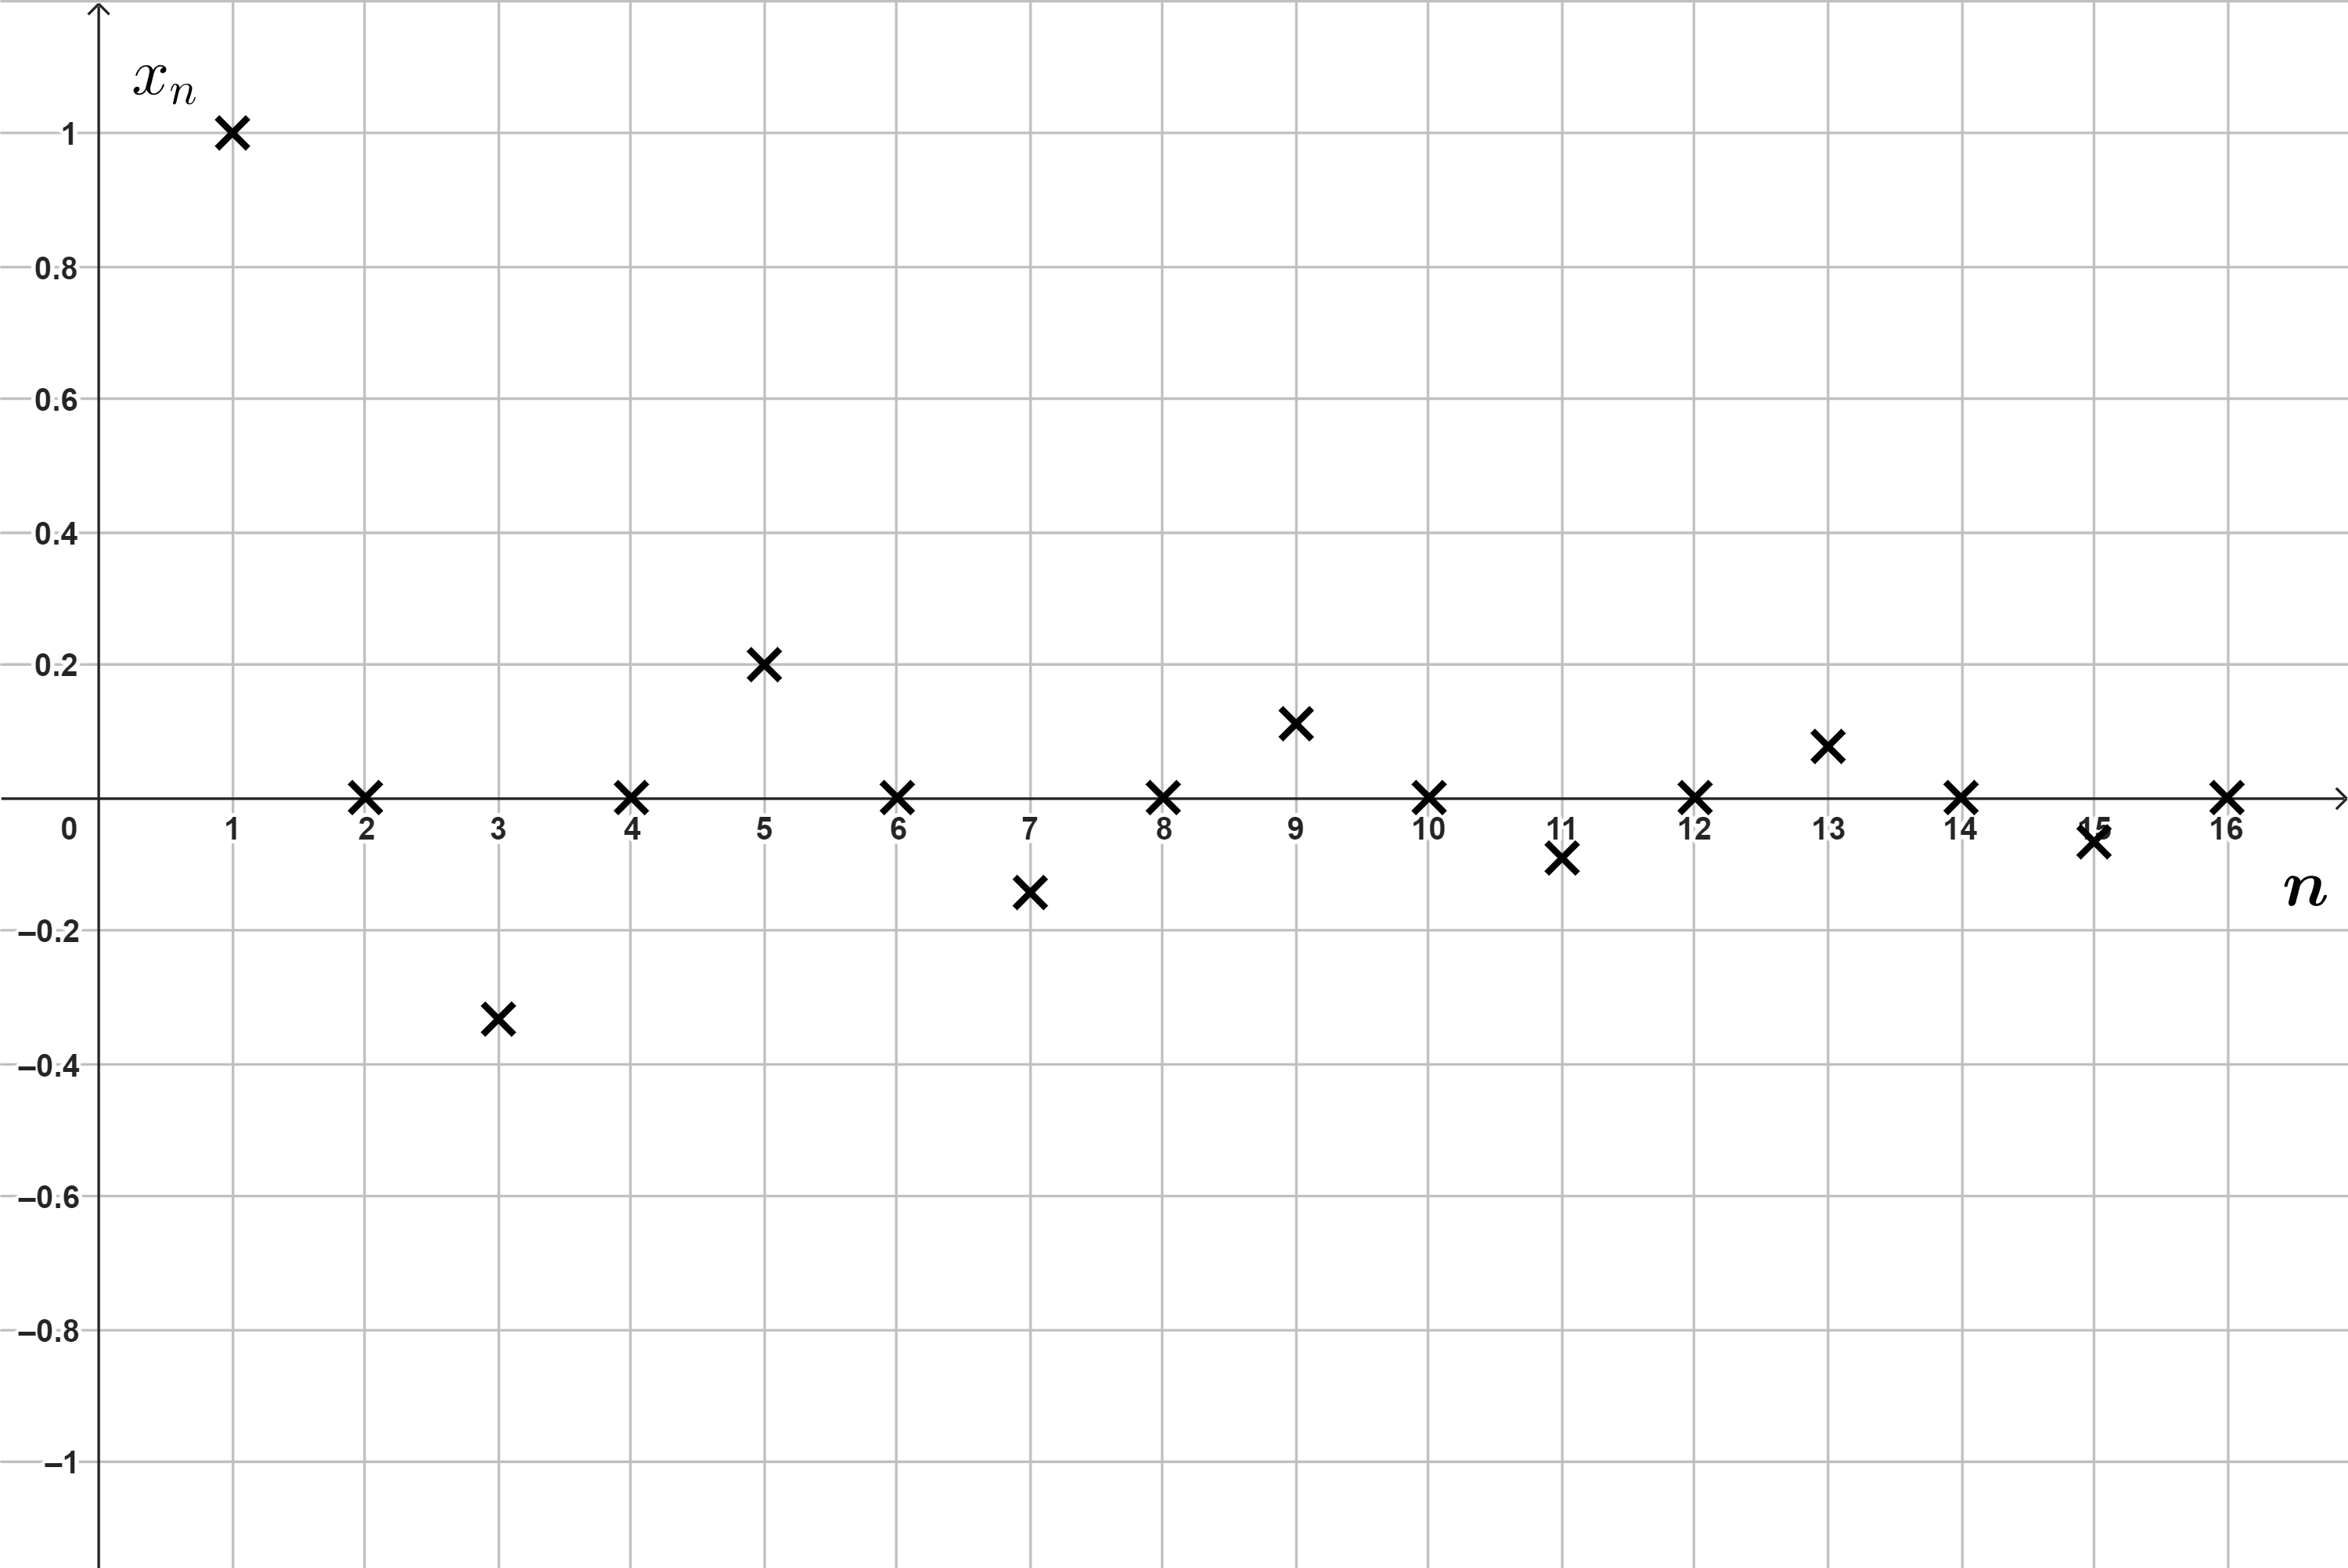
\includegraphics[scale=0.7]{Exercices/schema3.png}
    \caption{Representation des premiers termes de la suite $x_n=\frac{sin(n\frac{\pi}{2}}{n}$.}
    \label{fig:enter-label}
\end{figure}

\textbf{e)} Non. Il suffit de reprendre la définition de limite de suite pour s'en convaincre. Supposons qu'une suite $x_n$ converge vers $l$. On sait alors que quelque soit le $\epsilon$, on peut trouver un $N$ tel que $n \geq N \Rightarrow |x_n - l| < \epsilon$. \\
Pour rappel, une sous-suite est définie par $x_{n_k}$ avec $n_k = \phi(k), \ \forall k \in \Nn$, où $\phi: \Nn \rightarrow \Nn$ est une fonction strictement croissante. La suite des $n_k$ étant strictement croissante, on sait que pour tout $N$ qui satisfait $n \geq N \Rightarrow |x_n - l| < \epsilon$ dans la suite originale $x_n$, on pourra trouver un $K$ tel que $k \geq K \Rightarrow n_k \geq N$ et donc $|x_{n_k} - l| < \epsilon$.

\textbf{Principe des deux gendarmes}\\

\textbf{a)} On peut par exemple prendre $v_n = -\frac{1}{n}$ et $w_n = \frac{1}{n}$, car $-1 \leq sin(\frac{n \pi}{2}) \leq 1$. \\


\textbf{b)} Puisque $\lim_{n\rightarrow\infty}v_n=\lim_{n\rightarrow\infty}w_n=l$, on peut trouver $n_0\in\Nn$, tel que:
\begin{equation*}
    v_n-l>-\varepsilon \quad et \quad w_n-l<\varepsilon, \quad \forall n \geq n_0.
\end{equation*}
Alors on a 
\begin{equation*}
    -\varepsilon<v_n-l\leq y_n-l \leq w_n-l < \varepsilon, \quad \forall n \geq n_0,
\end{equation*}
et ainsi $\lim_{n\rightarrow\infty}y_n=l.  $ \\

\faLightbulbO \quad \fbox{\textbf{Discutez}} Il est plus facile de commencer par borner le dénominateur dans le présent exemple:
\begin{equation}
    n-1 \leq n + sin(n) \leq n+1 \Rightarrow \frac{1}{n+1} \leq \frac{1}{n + sin(n)} \leq \frac{1}{n-1},
\end{equation}
où on utilise le fait que l'inversion des members d'une inéquation change le sens de l'inégalité à condition que les membres soient positifs.

\end{exercice}

\begin{exercice}[Suite de Cauchy]
    
\textbf{a)} Pour $n,m \geq 1$, l'inégalité triangulaire donne:
\begin{equation}
    |x_n - x_m| = \Bigl\lvert\frac{(-1)^n}{n} - \frac{(-1)^m}{m}\Bigl\rvert \leq \frac{1}{n} + \frac{1}{m},
\end{equation}
ce qui montre que $x_n$ est une suite de Cauchy. En effet, pour un $\epsilon$ donné, prenons $N \in \Nn$ tel que $N > 2/\epsilon$. Alors,
\begin{equation}
    |x_n - x_m| \leq \frac{1}{n} + \frac{1}{m} \leq \frac{\epsilon}{2} + \frac{\epsilon}{2} = \epsilon, \quad \forall n,m \geq N.
\end{equation}
\\


\begin{figure}[H]
    \centering
    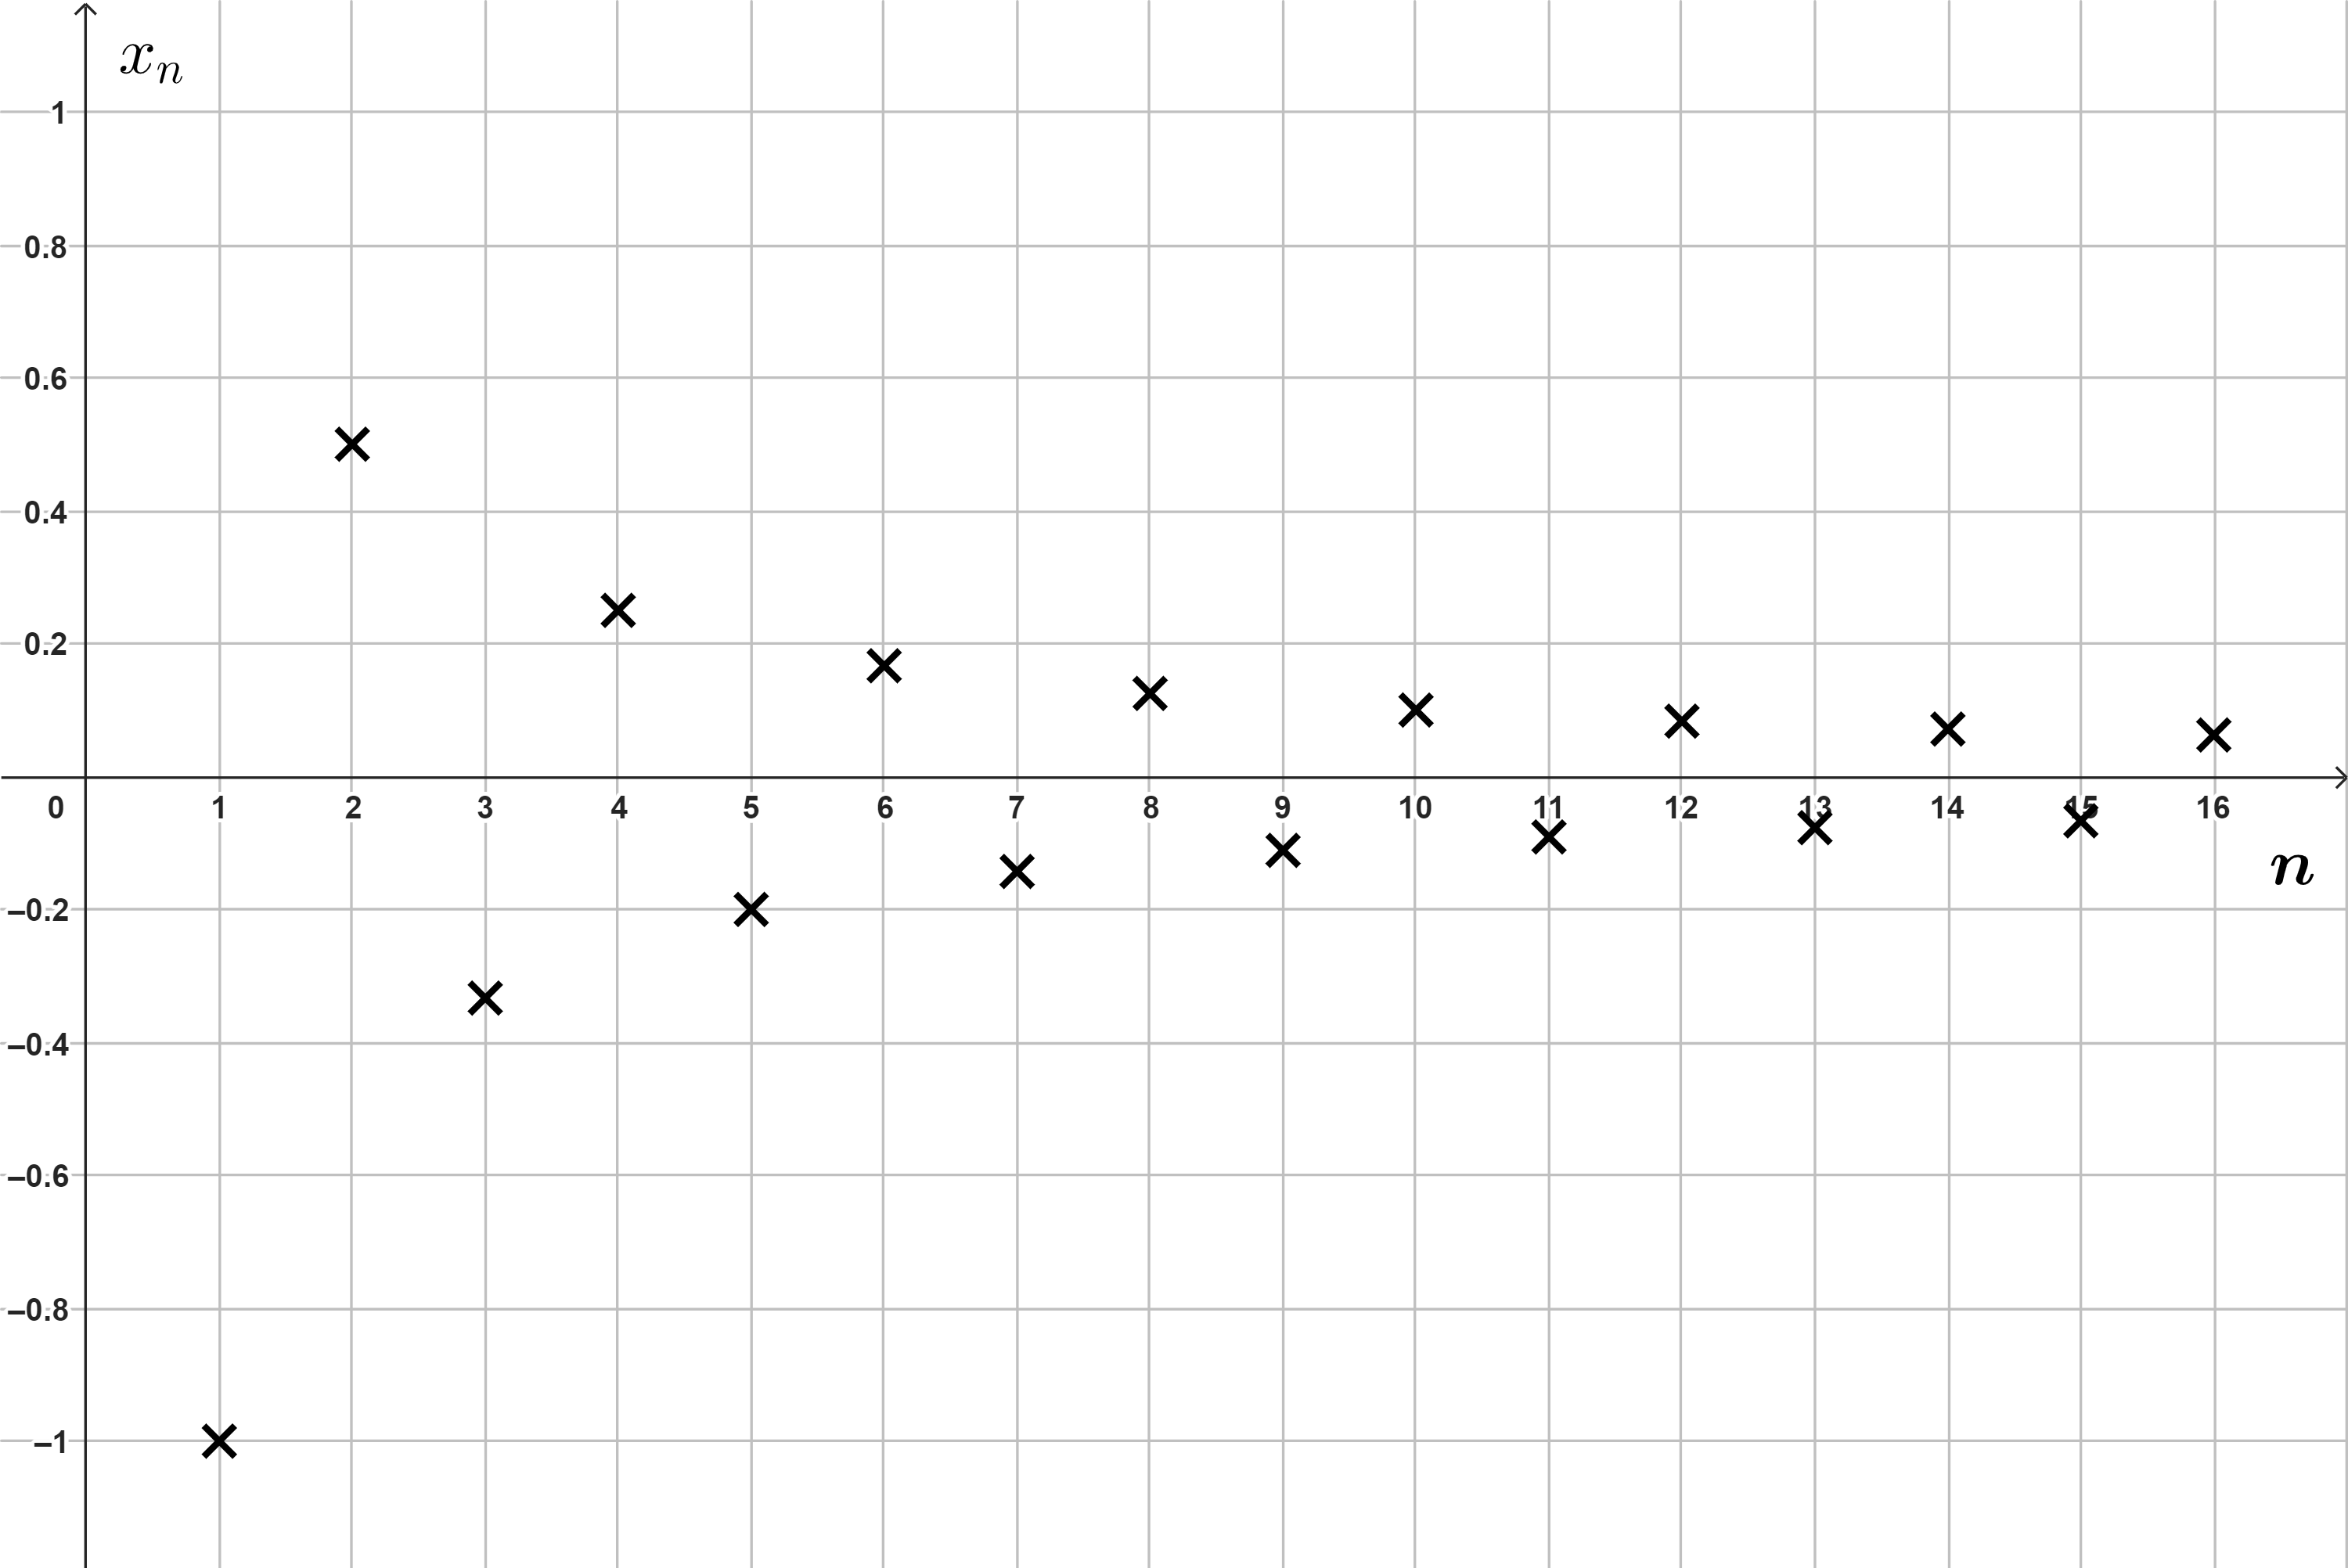
\includegraphics[scale=0.7]{Exercices/schema4.png}
    \caption{Representation des premiers termes de la suite $x_n=\frac{(-1)^n}{n}$}
    \label{fig:enter-label}
\end{figure}

\textbf{b)} Comme indiqué dans l'indice, il s'agit de montrer qu'une suite non bornée n'est pas de Cauchy.
Soit une suite $(x_n)$ de Cauchy non bornée, cela implique que $ \exists \  (|x_{n_k}|)$, une sous-suite, qui tend vers $\infty$. 
Donc, pour un $\varepsilon$ fixe, il existe un rang $N$ tq pour $m,n_k>N$: 
\begin{equation}
        |x_{n_k}-x_m|<\varepsilon.
\end{equation}
Or, si l'on fixe $m$ on a que $||x_{n_k}|-|x_m| |\to \infty (n\to \infty )$ et $||x_{n_k}|-|x_m| |\leq |x_{n_k}-x_m|<\varepsilon$ d'où la contradiction. \\

On vient donc de montrer qu'une suite non bornée ne peut pas être de Cauchy. Par conséquent, toute suite de Cauchy est forcément bornée. \\

\faLightbulbO \quad \fbox{\textbf{Discutez}} Non. Notons la proposition ``la suite est de Cauchy" A, et la proposition ``la suite est bornée" B. L'affirmation à prouver est donc $A \Rightarrow B$, soit en français ``si A est vrai, alors B est forcément vrai aussi". \\
Cette affirmation est équivalente à ``si B est faux, alors A est forcément faux aussi": $\neg B \Rightarrow \neg A$, où $\neg$ est le symbole de négation. On pourrait lire cela ``si B est faux alors le contraire de A est vrai", soit ``si suite bornée est faux (suite non bornée), alors le contraire de suite de Cauchy (la contradiction de suite de Cauchy, d'où le nom de démonstration par contradiction) est vrai".\\
Ce n'est en revanche pas équivalent à ce qui est proposé dans cet exercice: $\neg A \Rightarrow \neg B$ (soit ``si A est faux, alors B est forcément faux aussi") n'est pas équivalent à $A \Rightarrow B$!
\end{exercice}
\newpage
\begin{exercice}
    Posons tout d'abord \[(y_n)\subset \R : y_n = \cos{\frac{2\pi n^3+2}{n^2}}-1.\] \\
    Puis, puisque pour tout $a,b \in \R$, on a \[\cos a - \cos b = -2\sin{\frac{a+b}{2}}\,\sin{\frac{a-b}{2}},\] \\ 
    on montre facilement que
    \begin{align*}
        \left|\cos a - \cos b\right| &= 2\left|\sin{\frac{a+b}{2}}\right|\left|\sin{\frac{a-b}{2}}\right| \\ \\ &\leq 2\left|\sin{\frac{a-b}{2}}\right|.
    \end{align*}
   On trouve alors $\forall n \geq 1$: 
   \begin{align*}
       |y_n| = \left|\cos{\frac{2\pi n^3 + 2}{n^2}}- 1 \right| &=  \left|\cos{\frac{2\pi n^3 + 2}{n^2}}- \cos 2\pi n\right| \\ \\ 
       &\leq 2\left|\sin{\frac{\frac{2\pi n^3+2}{n^2}- 2\pi n}{2}}\right|. \\
   \end{align*}
    On peut maintenant conclure en se souvenant que $|\sin(t)| \leq |t|$ pour tout $t$ réel. \\ \\ En effet, 
    \begin{align*}
        |y_n| \leq 2\left|\sin{\frac{\frac{2\pi n^3+2}{n^2}- 2\pi n}{2}}\right| &\leq \left|\frac{2\pi n^3 + 2}{n^2} - 2\pi n\right| \\ \\
        &= \left|\frac{2}{n^2}\right| = \frac{2}{n^2} \\
    \end{align*}
    Ainsi, soit $\varepsilon > 0,$ si on choisit $N > \frac{\sqrt{2}}{\sqrt{\varepsilon}}$, on a bien pour tout $n \geq N$ \[|y_n| = \left|\cos{\frac{2\pi n^3 + 2}{n^2}}- 1 \right|< \frac{2}{n^2} < \frac{2}{N^2} < 2\left(\frac{\sqrt{\varepsilon}}{\sqrt{2}}\right)^2 =\varepsilon. \] \\
    D'où, \[\lim_{n \to \infty} \cos{\frac{2\pi n^3 + 2}{n^2}} = 1.\]
\end{exercice}

\begin{exercice}
    On a que 
    \begin{equation}
         \sin(\pi \sqrt{4 n^2+n})=\sin(\pi \sqrt{4 n^2+n} -2\pi n)  
    \end{equation}

    Or il apparait que :
    \begin{equation}
        \lim_{n\to \infty} \sqrt{4 n^2+n} -2 n= \lim_{n\to \infty} \dfrac{n}{\sqrt{4 n^2+n} +2 n}=\dfrac{1}{4}.
    \end{equation}

    Donc, 
    \begin{equation}
       \lim_{n\to \infty}  \sin(\pi \sqrt{4 n^2+n})=\sin(\dfrac{\pi}{4}).
    \end{equation}
\end{exercice}

\end{document}